\chapter{GUI application}

This milestone covers the development effort for implementing stage \ref{num:stage9} described in \Nameref{sec:developmentStages}.

\section{AvaloniaUI}

As decided in the project planning milestone (see chapter \ref{chap:evalProjPlan}), AvaloniaUI will be used as the \ref{itm:gui} framework.
Because AvaloniaUI uses \ref{itm:xaml} for defining the \ref{itm:ui} and utilizes \ref{itm:mvvm} as its architectural pattern, it was not too difficult to us it thanks to previous experience with \ref{itm:wpf} (Microsoft's official \ref{itm:gui} framework).

The only drawback of the framework is that it still does not have a stable release. This entails unreliability of the framework and possibility of breaking changes. For example, AvaloniaUI version 0.10.15 broke \ref{itm:ui} components for displaying images. Nevertheless, the it is backed-up by a passionate community of developers, that ensure any issues are resolved quickly.

The open source community added great value to the framework by developing additional libraries such as \textbf{AvaloniaBehaviors}, or \textbf{FluentAvaloniaUI}, both of which are used by the project. The former extends missing features for manipulating the \ref{itm:ui} based on defined triggers. The latter provides the FluentUI theme for AvaloniaUI. FluentUI is Microsoft's modern design system, that can be seen utilized across all of its applications. By default, the framework also uses FluentUI; however, it is outdated, or doesn't style all components. So, the \textbf{FluentAvaloniaUI} library is essential to have a modern design.

\section{Decoupling via MVVM}

Avalonia UI is a wonderful \ref{itm:gui} framework; however, it is not a first-party Microsoft product - this poses a higher risk of project abandonment. Moreover, users of the ModularDoc might not like Avalonia UI, and could even wish to have the tool hosted online in an \ref{gloss:aspnetcore} web application. Doubling down on agenda of a highly configurable tool results in an application which has its business logic completely independent from the \ref{itm:ui} framework.
This can be achieved using \ref{itm:mvvm} in combination with a \ref{itm:di} framework like Autofac.

\ref{itm:mvvm} (Model, View, View Model) allows natural decoupling of the \ref{itm:ui} (View), from the business logic (View Model) and data (Model). However, \ref{itm:mvvm} alone still introduces some coupling of the \ref{itm:ui} to the host application, as it must still reference the specific views for, e.g., navigation. Such references can be decoupled by abstracting each view with its interface representation. The specific views would then be provided via Autofac. This allows painless swapping of views either based on Avalonia UI, or some other framework.

To take it a step further, the view models can also be abstracted in the same exact way and provided via Autofac. In this case the benefit is higher application testability, as abstracted view models can be mocked.

\section{Application structure}

The \ref{itm:gui} application serves only as a configuration creator for the available plugins. Thus, the application requires minimum work on the \ref{itm:ui} side and will consist of the following pages:
\begin{itemize}
    \item Home page.
    \item Settings.
    \item About.
    \item Configuration stepper.
    \item Finalizer.
\end{itemize}

\subsection{Home page}

The home page presents the user with the available plugins. The \ref{itm:ux} is simplistic, as the user should only select the desired plugin, see its description, and decide whether they wish to use said plugin, or cancel.
Additionally, the user may wish to load a previously created configuration, so an option for loading that is available.
In case the application has a larger amount of plugins to offer, the user can search for the desired one via the search filter.

\subsubsection{Mock}

\begin{figure}[H]
    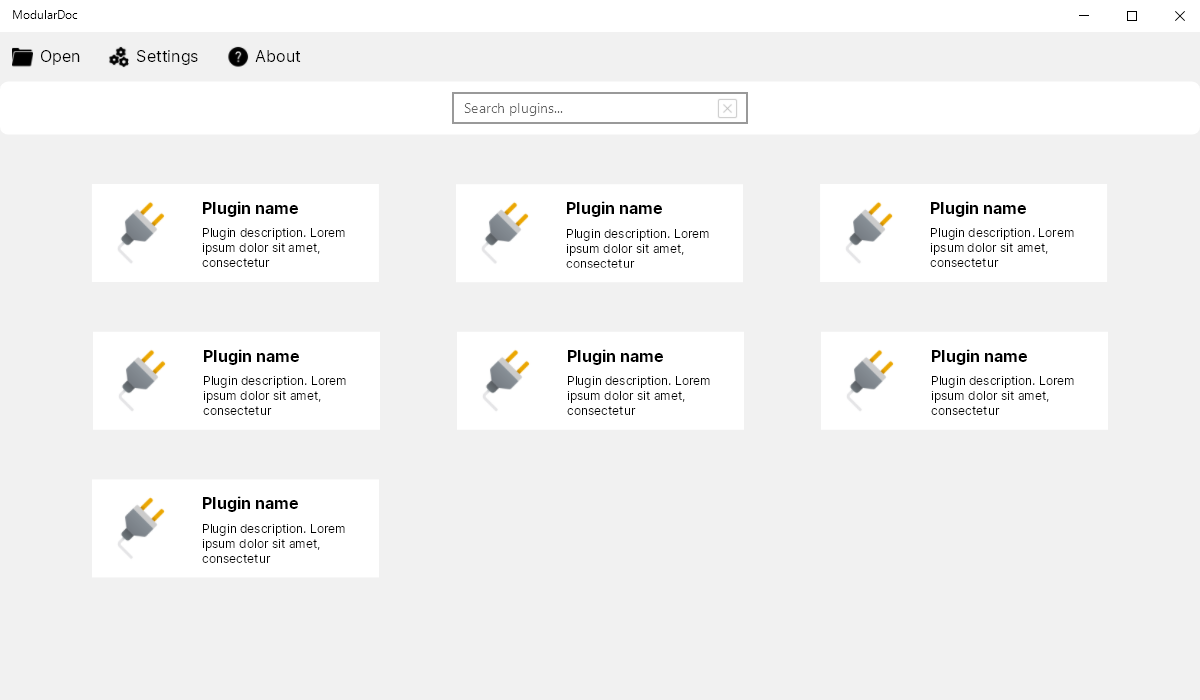
\includegraphics[width=\linewidth]{img/mockHome.png}
    \label{fig:homePage}
    \caption{Documentation generator home page}
\end{figure}

\begin{enumerate}
    \item Open button for loading previously defined configurations
    \item Settings button for navigating to the settings page
    \item About button for displaying information about the application
    \item Search entry for filtering the available plugins
    \item One of the available plugins with its icon, title, and short description
\end{enumerate}

\begin{figure}[H]
    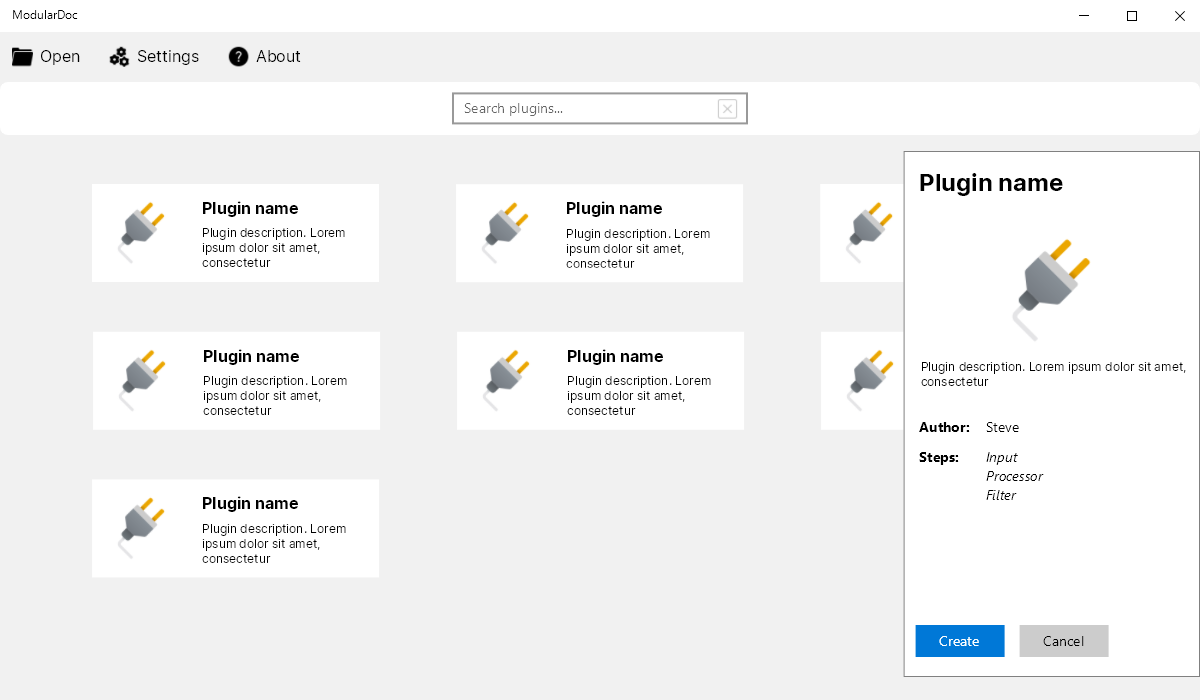
\includegraphics[width=\linewidth]{img/mockHome-PluginSelected.png}
    \label{fig:homePagePluginSelected}
    \caption{Documentation generator home page with a plugin selected}
\end{figure}

\begin{enumerate}
    \item Selected plugin title
    \item Selected plugin icon
    \item Author information
    \item Steps within said plugin
    \item Button for creating a configuration using the selected plugin
    \item Button for closing the selected plugin panel
\end{enumerate}

\subsection{Settings}

The settings page allows the user to configure the application. Since adding multicultural support would add more complexity to the project, the only setting provided on this page is a toggle between the light and dark mode themes.

\subsubsection{Mock}

\begin{figure}[H]
    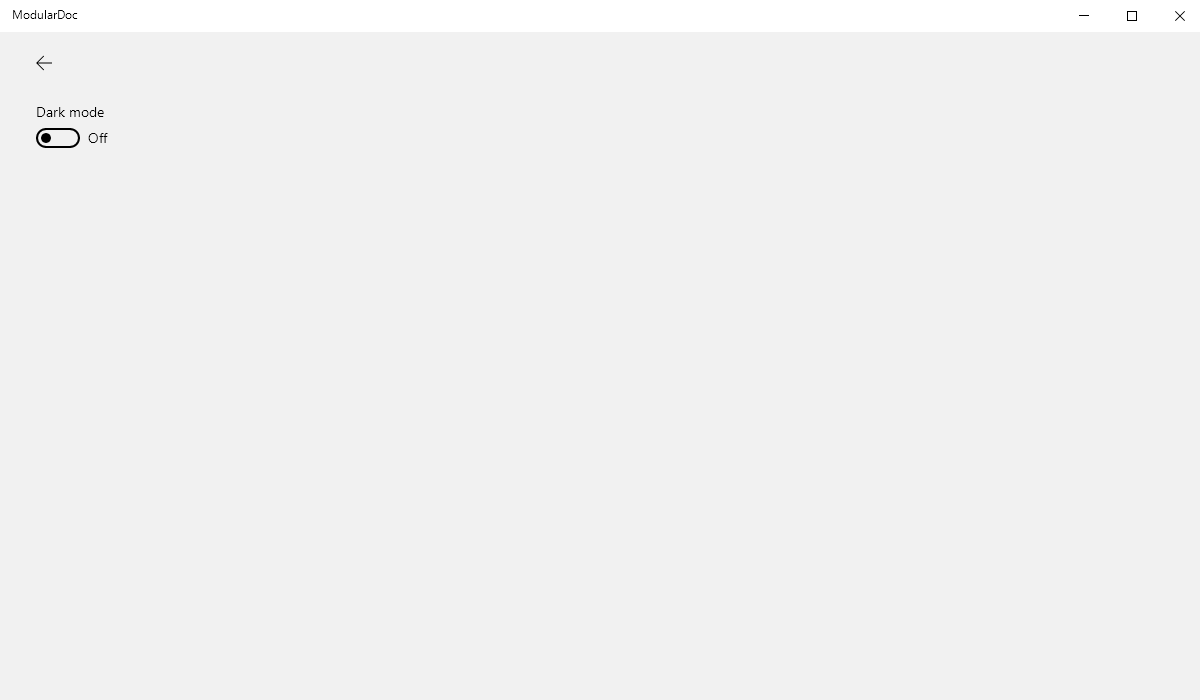
\includegraphics[width=\linewidth]{img/mockSettings.png}
    \label{fig:settingsPage}
    \caption{Documentation generator settings page}
\end{figure}

\begin{enumerate}
    \item Back button for navigating back to the home page
    \item Toggle switch for changing the theme from light mode to dark mode
\end{enumerate}

\subsection{About}

The about page would present the user with necessary information about the application, references to used libraries, and possibly usage instructions. However, the content of this page was neither designed, nor prepared, as it had a low priority and was left out of this development phase.

\subsection{Configuration stepper}

The configuration stepper is responsible for displaying configuration steps provided by the selected plugin. The \ref{itm:ui} of each step is provided by the plugin; thus, this page's design is only concerned about properly displaying the steps, and controls for navigating between them.

\subsubsection{Mock}

\begin{figure}[H]
    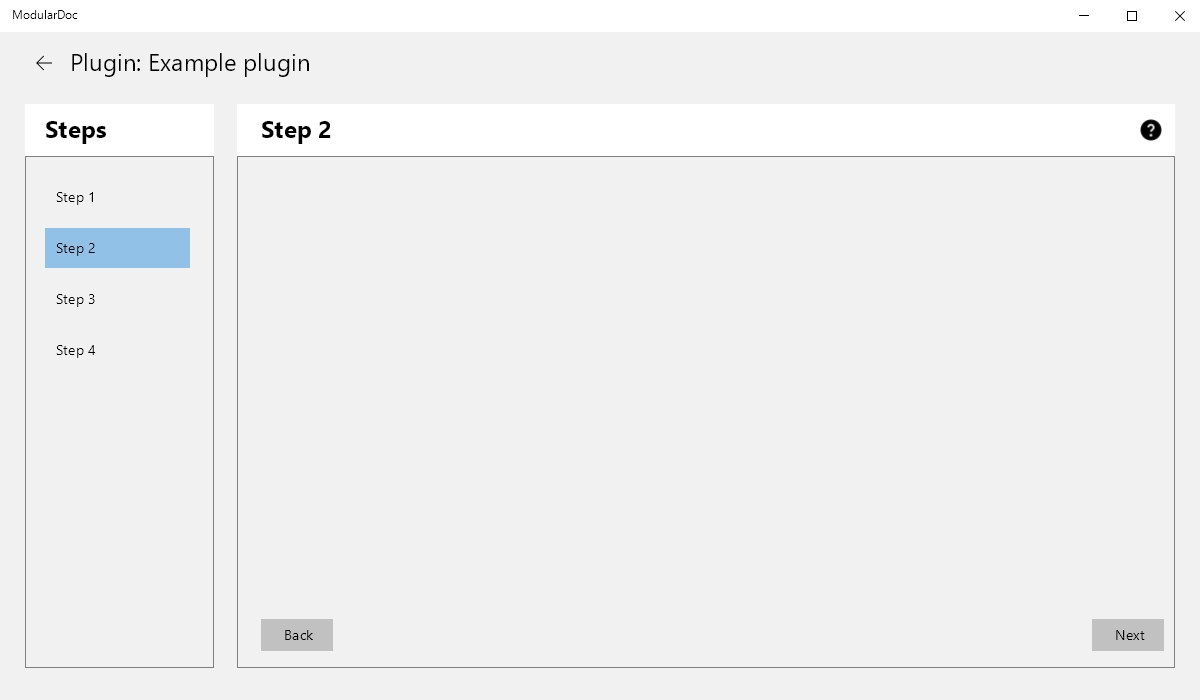
\includegraphics[width=\linewidth]{img/mockConfigurator.png}
    \label{fig:configuratorPage}
    \caption{Documentation generator configurator}
\end{figure}

\begin{enumerate}
    \item Title of the plugin
    \item List of steps provided by the plugin, with the current step highlighted
    \item The current step configuration title and view
    \item Information for the user to help them configure the step correctly
    \item Next button for navigating to the next step. Available only once the current step is correctly configured
\end{enumerate}

\subsection{Summary}

The summary is responsible for executing the selected plugin's configuration, either after loading it, or configuring it for the first time. It displays the progress of each plugin step, and logs what each process is doing.

\subsubsection{Mock}

\begin{figure}[H]
    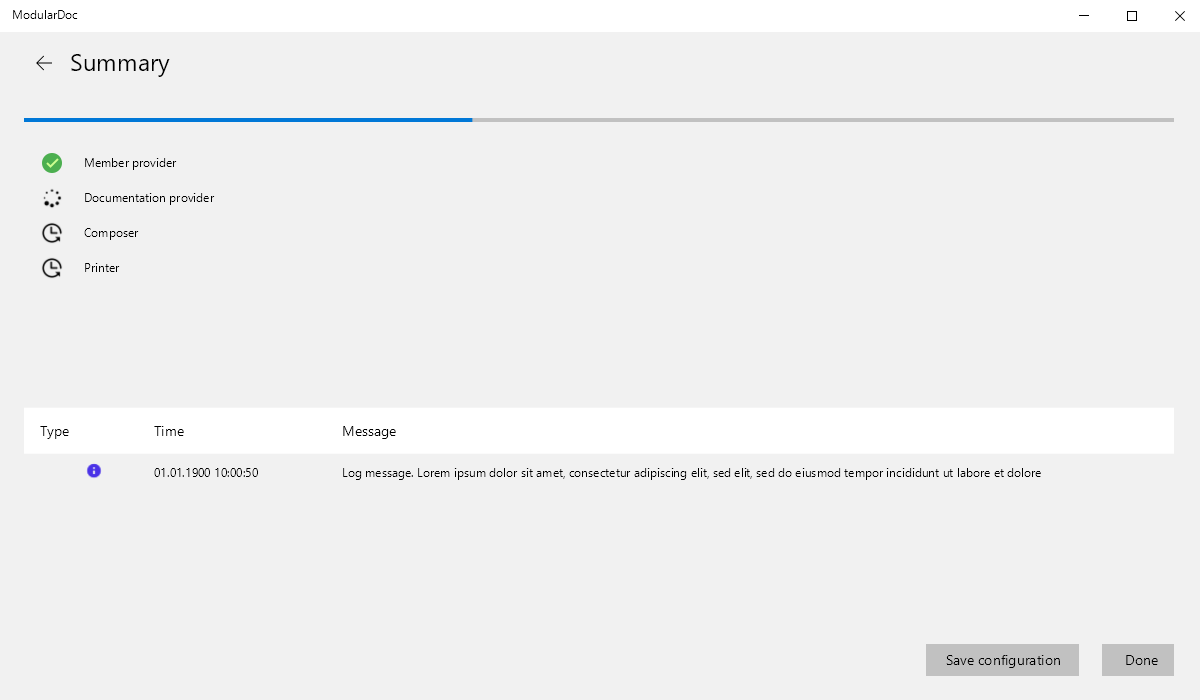
\includegraphics[width=\linewidth]{img/mockSummary.png}
    \label{fig:summaryPage}
    \caption{Documentation generator summary}
\end{figure}

\begin{enumerate}
    \item List of executed processes, their states
    \item Grouped logs on process sources and log types
    \item Button for saving the created configuration
    \item Button for closing the configurator
\end{enumerate}
